\subsubsection{Diamantstruktur}
Vi vet allerede at halvledere har 4 elektroner i valensbåndet.
Etter oktettregelen ønsker disse atomene
å fullføre sitt ytterste skall med 8 elektroner.
For å oppnå dette, danner de kovalente bindinger (elektronparbininger)
med andre atomer.
\\
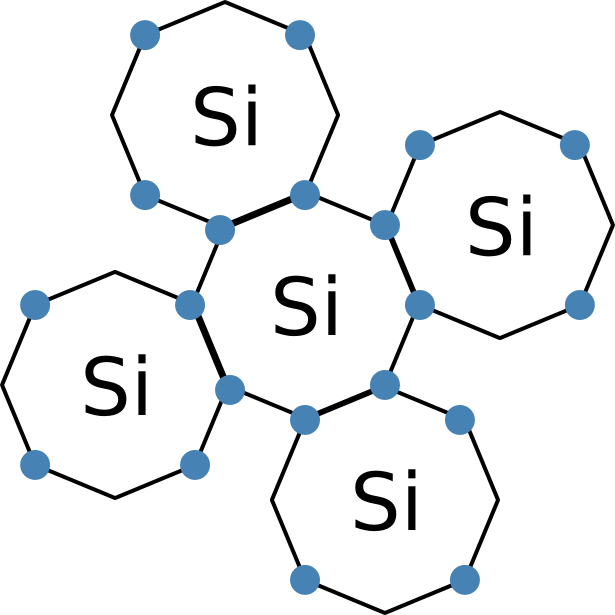
\includegraphics[width=0.5\textwidth]{./img/krystall.png}
\\
Silisiumatmoer danner en krystallstruktur.

\subsubsection{Ledning i rene halvledere}
Ved tilført energi (varme eller lys) kan elektronene løsrives
fra valensbåndet og bevege seg fritt i ledningsbåndet.
\\
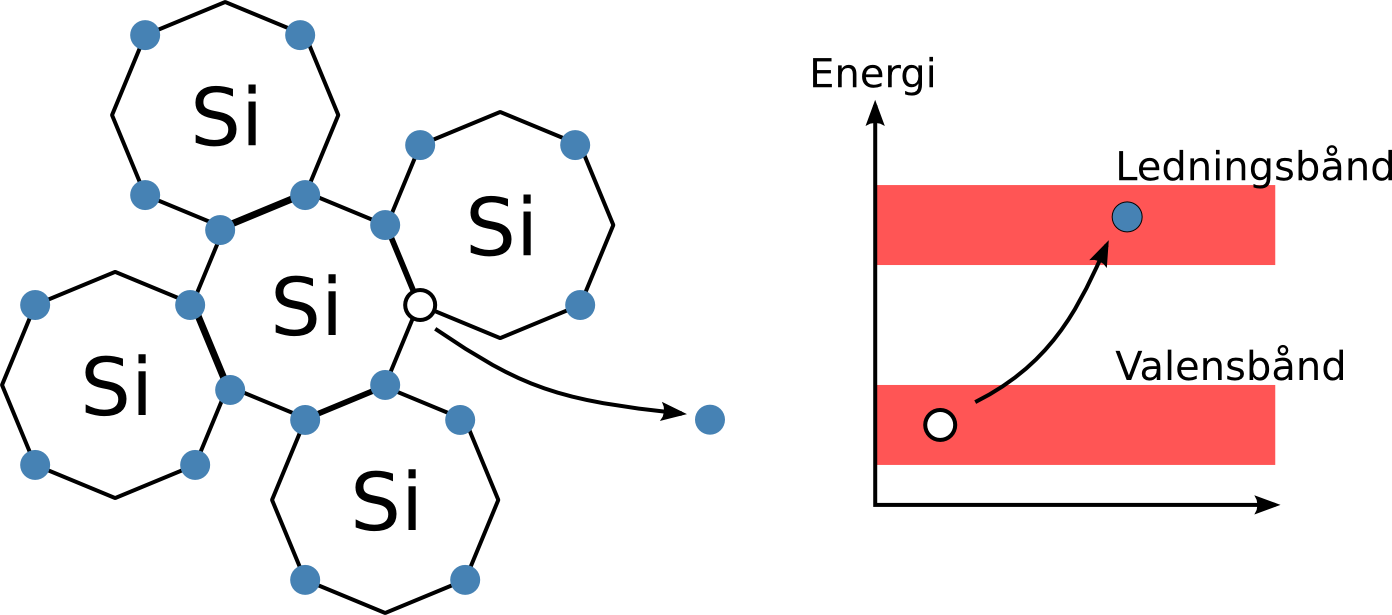
\includegraphics[width=\textwidth]{./img/krystall-ledning.png}
\\
Når elektroner faller tilbake igjen, ned i disse hullene,
kalles des rekombinasjon.
